\section{ Implementazione della dependency injection, i Services}
I componenti angular idealmente dovrebbero occuparsi esclusivamente di rendere possibile la user experience costruendo la vista applicativa e sfruttando il data binding per gestire la logica applicativa.
\newline
Per tutti i compiti esterni alla logica applicativa, Angular propone il concetto di Service.
\newline
I Service sono classi typescript descritte dal decorator @Injectable il cui compito è quello di occuparsi delle operazioni di utilità necessarie al funzionamento dei componenti.
Le operazioni gestite dai service possono includere:
\begin{itemize}
    \item Fetch dei dati da datasource esterne
    \item Logging delle operazioni o di debug
    \item Validazione del input utente
\end{itemize}
Grazie ai service è possibile rendere i componenti indipendenti da queste operazioni e rendere riusabile la struttura della vista utente. 
In questo modo i componenti non sono vincolati a particolari sistemi esterni, (ad esempio datasource) che possono avere concezioni di immagazzinamento dei dati differenti.

\subsection{Dependency Injection}
La dependency injection è una funzionalità diventata ormai fondamentale nelle applicazioni enterprise di grandi dimensioni, sia per testing del sistema sia per aumentare la riusabilità e la modularità delle applicazioni. Essa permette di rovesciare la logica di ottenimento delle dipendenze di un particolare componente sofware, liberando il componente dall'obbligo di reperire le dipendenze e delegando a altre entità il compito.
\begin{figure}[H]
    \centering
 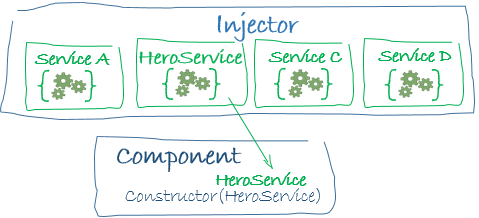
\includegraphics[scale=0.75]{resources/injector-injects.png}
\cite{angular-doc}
   \caption{rappresentazione oggetto Injector}
\end{figure}
La libreria Angular implementa questa funzionalità attraverso i service, essi possono essere richiesti dal costruttore di un componente e vengono forniti dal framework alla creazione dello stesso tramite un oggetto chiamato Injector, in questo modo il componente necessita solo di dichiarare il service di cui ha bisogno e non di definirne la logica di funzionamento o di occuparsi della sua creazione o istanziazione.
\newline
\newline
Un service, per poter essere iniettato all'interno di un componente necessita un provider che consente di definire la visibilità del service. 
Quest'ultima può essere:
\begin{itemize}
    \item A livello di componente, in questo caso per ogni istanza dello specifico componente viene creata un istanza del service
    \item A livello di ngModule, in questo modo viene creata una sola istanza per tutti i componenti che fanno parte di quel service
    \item A livello radice, in questa modalità viene creata una sola istanza del service, che viene resa disponibile a tutti i componenti interni all'applicazione
\end{itemize}
La capacità dei provider di limitare la visibilità dei service è fondamentale anche sotto un punto di vista di ottimizzazione delle prestazioni, in quanto consente di istanziare i service solo in caso si utilizzi il componente applicativo che ne ha un effettivo bisogno.
\newpage
